\documentclass[french,12pt]{exam}

%\printanswers

\usepackage{../../latex/macro_mealor}
\usepackage[utf8]{inputenc}
\usepackage[T1]{fontenc} % accents codés dans la fonte
%\usepackage{layout}
\usepackage{a4wide}
%\usepackage[french]{babel}
\usepackage{hyperref}

\usepackage{graphicx}
\usepackage{caption}

\usepackage{newpxtext,newpxmath}
\usepackage{siunitx}

%\setlength{\hoffset}{0pt}
%\setlength{\oddsidemargin}{-1cm}   % Marge gauche sur pages impaires
%\setlength{\evensidemargin}{-1cm}   % Marge gauche sur pages paires
%\setlength{\marginparwidth}{0cm}   % Largeur de note dans la marge
%\setlength{\textwidth}{16cm}   % Largeur de la zone de texte (17cm)
\setlength{\voffset}{0pt}   % Bon pour DOS
\setlength{\marginparsep}{0pt}   % Séparation de la marge
\setlength{\topmargin}{0cm}   % Pas de marge en haut
\setlength{\headheight}{0cm}   % Haut de page
\setlength{\headsep}{0cm}   % Entre le haut de page et le texte
%\setlength{\footskip}{1cm}   % Bas de page + séparation
%\setlength{\textheight}{25.5cm}   % Hauteur de la zone de texte (25cm)

\usepackage{indentfirst}


\newcommand{\classurl}{\url{1}}
% #1 numéro de la feuille
% #2 titre de la feuille
\newcommand{\titre}[3] {%\textit{
  \begin{center}\textbf{\textsc{MEALOR II}}\\ \textit{Mécanique de l'endommagement et approche locale de la rupture}%\let\thefootnote\relax\footnotetext{\classurl} 
  \end{center}
 
  \noindent TD n\textdegree #1 \hfill  August 2023\\[-0.3cm]
  \rule{\linewidth}{.3mm}
  \vspace*{0.5pt}
  \begin{center}
    {
      \Large \bfseries { #2}
    }\\
    \vspace*{0.5cm}
	\large #3
    \vspace*{0.5cm}
  \end{center}
}

\usepackage{xcolor}
\definecolor{Blue}{RGB}{0,68,170}
\SolutionEmphasis{\normalfont\color{Blue}}
\DeclareCaptionFont{blue}{\color{Blue}}

\newenvironment{objectifs}
    {\itshape\underline{Objectifs:}\begin{itemize}
    }
    { \itshape
    \end{itemize}
    }
    
\newcounter{Rfig}
\newenvironment{R_figure}
   {\begin{minipage}{\linewidth}\begin{center}\vspace{0.5mm}\stepcounter{Rfig}\addtocounter{figure}{-1}\renewcommand\thefigure{R-\arabic{Rfig}}
   \captionsetup{font=blue}}
   {\end{center}\vspace{0.5mm}\end{minipage}}
   
    
\newcounter{Rtab}
\newenvironment{R_table}
   {\begin{minipage}{\linewidth}\begin{center}\vspace{0.5mm}\stepcounter{Rtab}\addtocounter{table}{-1}\renewcommand\thetable{R-\arabic{Rtab}}
   \captionsetup{font=blue}
}
   {\end{center}\vspace{0.5mm}\end{minipage}}
   
      
\graphicspath{{./pic/}}
\usepackage{float}

\newcommand{\todo}[1]{\textbf{\textcolor{red}{[ToDo: #1]}}}
\begin{document}
\thispagestyle{empty}
\titre{3}{Rupture ductile : homogénéisation de matériaux poreux}{Jérémy Hure, Djimédo Kondo, Jérémy Bleyer}

\begin{objectifs}
\item Obtenir un critère de plasticité pour matériaux poreux dans le cadre de la modélisation de la rupture ductile
\item Analyser ce critère et dériver l'évolution de la porosité
\item Discuter des effets d'anisotropie
\end{objectifs}

\section{Position du problème}
On cherche ici à redériver les étapes de construction du modèle de Gurson dans le cas d'un matériau poreux \textit{cylindrique} (Figure \ref{fig1}).

\begin{figure}[H]
  \centering
  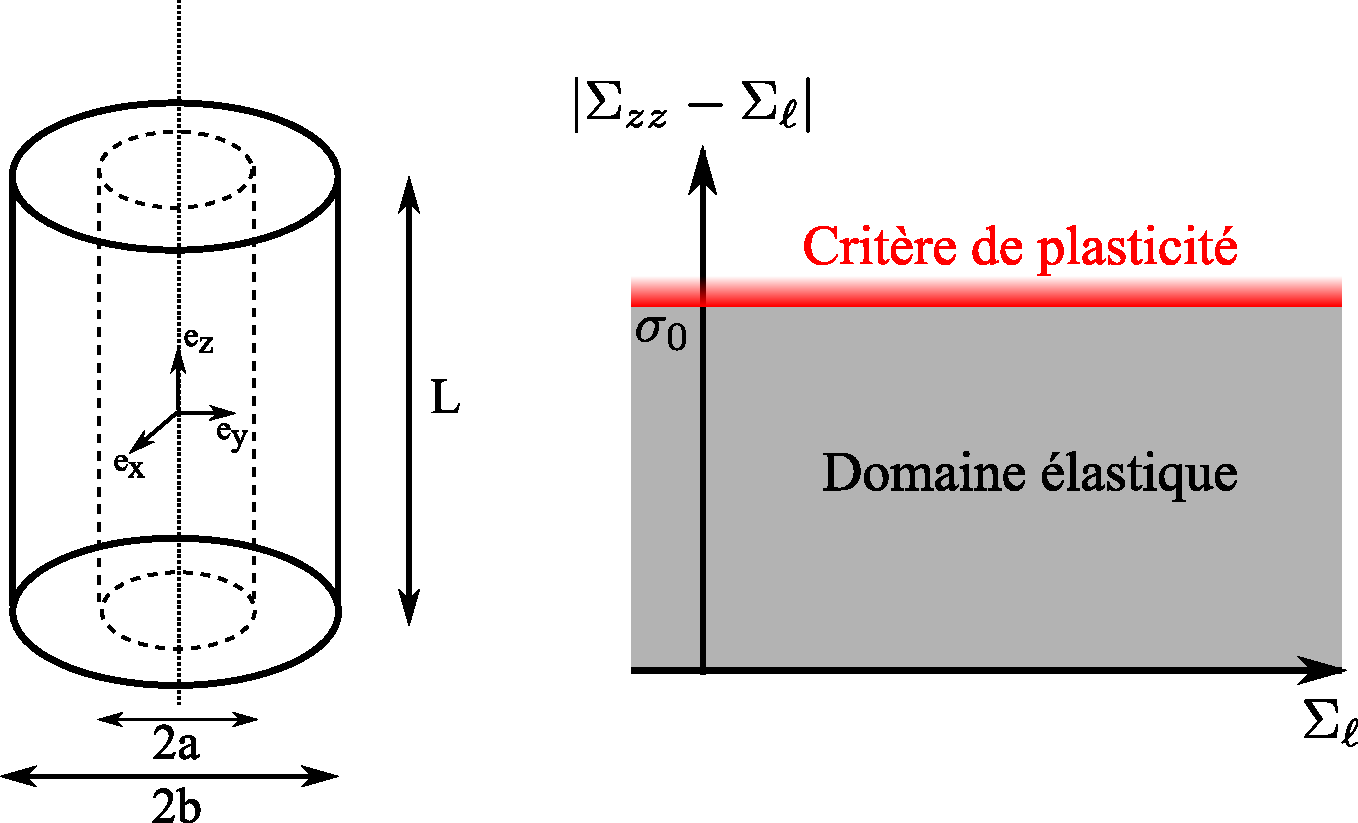
\includegraphics[height = 7cm]{homoMEALOR.pdf}
\caption{Géométrie considérée et critère de plasticité}
\label{fig1}
\end{figure}


Le point de départ est de considérer, pour la matrice, le \textbf{critère de plasticité de von Mises} qui s'écrit:
\begin{equation}
  \phi\left( \td{\sigma}   \right) =  \sigma_{eq} - \sigma_0 \leq 0 \hspace{2cm} \sigma_{eq} = \sqrt{\frac{3}{2} \td{s} \cdot \td{s}} \ \ \ \ \mathrm{avec} \ \ \ \ \td{s} = \tsigma - \frac{1}{3} \mathrm{tr}\tsigma \td{I}
  \label{eq1}
\end{equation}
La déformation plastique se produit quand le critère est atteint, \textit{i.e.}, $\phi = 0$. Dans tout l'exercice, l'écrouissage n'est pas pris en compte ($\sigma_0 = \text{cste}$) et l'élasticité est ignorée, ce qui correspond à un matériau dit \textit{rigide parfaitement plastique}.

La loi d'écoulement plastique associée permet d'obtenir le taux de déformation plastique:
\begin{equation}
  \td{d} = d_{eq} \frac{3 \td{s}}{2 \sigma_0}  \hspace{2cm} d_{eq} = \sqrt{\frac{2}{3}\td{d} \cdot \td{d} }
  \label{eq200}
\end{equation}
conduisant à la dissipation plastique $\sigma_0d_{eq}(\td{v})$ pour un champ $\td{v}$ incompressible, c'est-à-dire tel que $\mathrm{tr}(\td{d})=0$.\\

Afin de déterminer un critère de plasticité macroscopique du milieu poreux, la géométrie présentée sur la Fig.~\ref{fig1} est considérée, à savoir un cylindre creux de hauteur $L$, de rayons intérieur $a$ et extérieur $b$. La porosité, définie comme le rapport entre le volume de la cavité et le volume total est noté $f = (a/b)^2$. Enfin, on note $V$ le cylindre de rayon $b$ (incluant donc le pore) et $\partial V$ le bord extérieur de rayon $b$.

On \textbf{impose} sur la frontière extérieure du cylindre des conditions aux limites homogènes en taux de déformation:
\begin{align}
\td{v}(\td{x}) &= \td{D}\cdot\td{x} \quad \text{pour tout }\td{x}\in \partial V \label{eq:CL}
\end{align}
où $\td{D}$ est un paramètre de chargement donné de la forme suivante:
\begin{equation}
\td{D} = D_{xx} (\td{e}_x \otimes \td{e}_x + \td{e}_y \otimes \td{e}_y) + D_{zz} \td{e}_z \otimes \td{e}_z \label{eq:D-GPS}
\end{equation}

Les conditions aux limite assurent alors que $\td{D}$ est le taux de déformation (plastique) macroscopique associé à tout champ de vitesse vérifiant \eqref{eq:CL}. De plus, en introduisant la contrainte macroscopique $\tSigma$, ces grandeurs macroscopiques sont reliées à leurs équivalents microscopiques par les relations suivantes:
\begin{align}
  \tSigma &= \frac{1}{V} \int_V \tsigma dV\\
  \td{D} &= \frac{1}{V} \int_V \td{d} \, dV \\
  &= \frac{1}{2V} \int_{\partial V} \left(\td{v} \otimes \td{n} + \td{n} \otimes \td{v}     \right) dS \label{eq:D-v-n}
\end{align}
avec $\td{v}$ le champ de vitesse et $\td{n}$ la normale extérieure à la surface.\\


\begin{questions}
\question Quel classe de matériaux poreux peut être représentée par cette géométrie ? Dans le cas de chargement axisymétrique, montrer que le critère de plasticité en l'absence de cavité, donné par le critère de von Mises de la matrice, correspond à la Fig.~\ref{fig1} où $\Sigma_\ell$ désigne la contrainte latérale dans le plan $(x,y)$.\\
\end{questions}

\begin{solution}
Le fait de considérer des pores cylindriques correspond à une idéalisation de cavités très allongées dans la direction $z$. Ce type de situation peut se rencontrer dans le cas de tôles d'aciers laminés à chaud.\\

En l'absence de cavité, le champ de contrainte est homogène et égal au champ macroscopique:
$$\td{\sigma} = \Sigma_{xx}\td{e}_x\otimes\td{e}_x + \Sigma_{yy}\td{e}_y\otimes\td{e}_y +  \Sigma_{zz}\td{e}_z\otimes\td{e}_z$$
avec $\Sigma_{xx}=\Sigma_{yy}=\Sigma_\ell$ pour un chargement axisymétrique. Dans ce cas, le déviateur est:
$$\td{s} = \dfrac{1}{3}(\Sigma_{\ell}-\Sigma_{zz})(\td{e}_x\otimes\td{e}_x + \td{e}_y\otimes\td{e}_y - 2\td{e}_z\otimes\td{e}_z)$$
De sorte que le critère s'exprime comme:
$$\sigma_{eq} = |\Sigma_\ell - \Sigma_{zz}| \leq \sigma_0$$
qui correspond bien au cylindre d'axe $\Sigma_{\ell}$ de la figure. Il s'agit d'un critère \textit{isotrope}.
\end{solution}

On rappelle que l'on cherche à obtenir le critère de plasticité du cylindre, c'est-à-dire l'équivalent de l'Eq.~\ref{eq1} pour les grandeurs macroscopiques $\tSigma$ et $\td{D}$ en présence d'une cavité. Pour cela, la théorie de l'analyse limite est utilisée. En pratique, celle-ci consiste à postuler un champ de vitesse $\td{v}$ admissible (dans un sens qui sera précisé par la suite), et à calculer la dissipation plastique associée:
\begin{equation}
  \Pi(\td{D}) = \frac{1}{V} \int_V \sigma_0 d_{eq}(\td{v}) \,dV
  \label{eq3}
\end{equation}

Sous certaines conditions (qui là-encore seront détaillées dans la suite), cette dissipation plastique permet d'évaluer la contrainte maximale admissible, c'est-à-dire le critère de plasticité macroscopique, par l'équivalence suivante:
\begin{equation}
  \tSigma \cdot \td{D} \leq \Pi(\td{D}) \quad \forall \td{D} \quad \Longleftrightarrow \quad \Phi(\tSigma) \leq 0 \label{eq2}
\end{equation}
où $\Phi$ désigne le critère de plasticité macroscopique. De plus, on peut montrer que la frontière $\Phi(\tSigma^*)=0$ du critère est décrite par les états de contrainte tels que:
\begin{equation}
\tSigma^*\cdot\td{D} = \Pi(\td{D}) \quad \Longleftrightarrow \quad \tSigma^* = \dfrac{\partial \Pi}{\partial \td{D}}
  \label{eq:plastic-boundary}
\end{equation}
La frontière est ainsi paramétrée par la valeur\footnote{En réalité, $\Pi(\td{D})$ étant homogène de degré 1, l'expression \eqref{eq:plastic-boundary} ne dépend pas de la norme de $\td{D}$ mais uniquement de sa direction.} de $\td{D}$.

\section{Champ de vitesse et dissipation plastique}

Afin d'obtenir une estimation du critère de plasticité, la première étape consiste donc à choisir un champ de vitesse pris sous la forme, initialement proposée par Gurson:
\begin{equation}
  \td{v} = v_r(r) \td{e}_r + v_z(z) \td{e}_z \label{eq:champ-vitesse}
\end{equation}

\begin{questions}
\question En imposant que le champ de vitesse soit incompressible, montrer que celui-ci est de la forme:\\
\begin{equation}
  \td{v} = \left( \frac{B}{r} -  \frac{A}{2}r \right)  \td{e}_r +  A z \td{e}_z 
\end{equation}
\textit{On pourra s'aider du formulaire rappelé à la fin du sujet.}

\begin{solution}
L'incompressibilité s'écrit ici:
$$\mathrm{tr}\td{d} = \divergence{\td{v}} = v_r'(r)+\dfrac{v_r(r)}{r}+v_z'(z)=0$$
Comme les deux premiers termes ne dépendent que de $r$ et le troisième que de $z$, ce dernier est nécessairement constant, c'est-à-dire: $v_z(z) = Az$. De plus, on a ainsi:
$$v_r'(r)+\dfrac{v_r(r)}{r}= \dfrac{1}{r}(rv_r)'=-A$$
Ce qui donne après intégration:
$$rv_r(r) = B -  \frac{A}{2}r^2$$
soit au final:
\begin{equation}
  \td{v} = \left( \frac{B}{r} -  \frac{A}{2}r \right)  \td{e}_r +  A z \td{e}_z 
\end{equation}
où $A$ et $B$ sont deux constantes indéterminées.
\end{solution}

\question Déterminer $A$ et $B$ en fonction des composantes de $\td{D}$ afin que ce champ vérifie les conditions aux limites imposées en \eqref{eq:CL}.
\begin{solution}
On doit avoir sur le bord extérieur:
\begin{align*}
\td{v}(\td{x}=b\td{e}_r+z\td{e}_z) &= \td{D}\cdot(b\td{e}_r+z\td{e}_z)\\
\left(\frac{B}{b}-\frac{A}{2}b\right)\td{e}_r + Az\td{e}_z &= b D_{xx}\td{e}_r + zD_{zz}\td{e}_z
\end{align*}
On en déduit:
$$
\boxed{
\begin{array}{l}
A = D_{zz}\\
B = b^2\left(D_{xx}+\frac{1}{2}D_{zz}\right)
\end{array}}
$$
On notera que si $\td{D}$ est purement déviatorique $(\mathrm{tr}(\td{D})=0$), alors $B=0$. $A$ est donc relié à la partie déviatorique et $B$ à la partie hydrostatique.
\end{solution}

\question Calculer le taux de déformation microscopique $\td{d}$ associé.
\begin{solution}
Le taux de déformation microscopique vaut:
$$\td{d} = \left(-\frac{A}{2}-\frac{B}{r^2}\right)\td{e}_r\otimes\td{e}_r + \left(-\frac{A}{2}+\frac{B}{r^2}\right)\td{e}_\theta\otimes\td{e}_\theta + A\td{e}_z\otimes\td{e}_z$$
On remarquera que si $B=0$, le champ déviatorique proposé est uniforme. On anticipe ici une faiblesse possible du choix initial pour le champ de vitesse.
\end{solution}

%On peut vérifier que l'on a bien 
%On constate donc que le terme en $A$ est homogène et est donc associé à un tenseur de déformation macroscopique de la forme $-\frac{A}{2}\td{1}_p + A\td{e}_z\otimes\td{e}_z$ où $\td{1}_p$ représente l'identité du plan $(\td{e}_x,\td{e}_y)$. 
%
%Le deuxième terme en $B$ est associé au champ de vitesse purement radial $\frac{B}{r}\td{e}_r$. Il est donc associé au tenseur de déformation donné par:
%\begin{align*}
%\frac{1}{2V} \int_{\partial V} \left(\td{v} \otimes \td{n} + \td{n} \otimes \td{v}     \right) dS &= \frac{1}{V}\int_{\partial V} \dfrac{B}{b} \td{e}_r\otimes\td{e}_r dS \\
%&= \dfrac{L B}{\pi b^2 L} \int_0^{2\pi}\td{e}_r\otimes\td{e}_r d\theta\\
%&= \dfrac{B}{b^2} \td{1}_p
%\end{align*}
%\textbf{Attention!} on ne peut utiliser directement l'intégrale de volume entre $a$ et $b$ car le champ ne peut pas être prolongé dans le pore n'importe comment, en particulier pas par $\td{d}=0$. Il est donc plus sûr d'utiliser la relation \eqref{eq:D-v-n} qui ne dépend pas de la façon dont on prolonge le champ dans le bord, cf. Leblond, J. B. "Mécanique de la rupture fragile et ductile, 2000.
%
%On a donc au final:
%$$\td{D} = \left(\dfrac{B}{b^2}- \dfrac{A}{2}\right)\td{1}_p + A\td{e}_z\otimes\td{e}_z$$
%On note que si $B=0$, le chargement macroscopique est purement déviatorique tandis que si $A=0$, on a un chargement purement hydrostatique dans le plan.
%\end{solution}

%Ce champ de vitesse est \textbf{cinématiquement admissible} avec un tenseur des déformations et \textbf{plastiquement admissible}, \textit{i.e.}, est compatible avec la plasticité de von Mises qui impose un écoulement incompressible. De plus, il est possible de montrer que $\td{v}(\partial V) = \td{D} \cdot \td{x}$, avec $\td{x}$ le vecteur position, ce qui correspond à des conditions aux limites de type \textbf{homogène au bords en déformation}. Ces trois conditions justifient théoriquement l'utilisation de l'analyse limite (Eq.~\ref{eq2}). %Dans la suite, on fait l'hypothèse que $A \geq 0$ et $B \geq 0$.\\


\question \'Evaluer la puissance des efforts extérieurs $\tSigma \cdot \td{D}$ en fonction de $A$ et $B$. On pourra poser $(\Sigma_{xx}+\Sigma_{yy})/2= \Sigma_\ell$.
\begin{solution}
La puissance s'écrit ici:
\begin{align*}
\tSigma \cdot \td{D} &= \Sigma_{xx}D_{xx}+\Sigma_{yy}D_{xx}+\Sigma_{zz}D_{zz}\\
&= \left(\dfrac{B}{b^2}- \dfrac{A}{2}\right)(\Sigma_{xx}+\Sigma_{yy})+\Sigma_{zz}A \\
&= \dfrac{B}{b^2}2\Sigma_\ell + (\Sigma_{zz}-\Sigma_\ell)A
\end{align*} en notant $(\Sigma_{xx}+\Sigma_{yy})/2= \Sigma_\ell$.
\end{solution}

\question \'Etablir l'expression de la dissipation plastique $\Pi$ (Eq.~\ref{eq3}) sous la forme d'une intégrale qu'on ne cherchera pas à calculer pour l'instant.
\begin{solution}
On a ici:
\begin{align*}\Pi(\td{D}) &= \frac{1}{V} \int_V \sigma_0 d_{eq}(\td{v}) \,dV \\
&= \frac{1}{\pi b^2 L} \left(\int_0^L dz\right)\left(\int_0^{2\pi} d\theta\right)\int_a^b \sigma_0 d_{eq}(v) rdr\\
&= \frac{2}{b^2} \int_a^b \sigma_0 d_{eq}(v) rdr
\end{align*}
où:
$$d_{eq} = \sqrt{\dfrac{2}{3}}\sqrt{d_{rr}^2+d_{\theta\theta}^2+d_{zz}^2} = \sqrt{\dfrac{4}{3}\dfrac{B^2}{r^4}+A^2}$$
\end{solution}
\end{questions}

\section{Estimations}
Avant d'évaluer cette intégrale dans le cas général, nous considérons deux cas de chargement particuliers, à savoir $(B = 0, A \neq 0)$ et  $(B \neq 0, A = 0)$.\\

\begin{questions}
\question En calculant la dissipation plastique $\Pi$ et explicitant l'Eq.~\ref{eq2} dans chacun de ces cas, déterminer les estimations du critère de plasticité associées.
\begin{solution}
Dans le cas $B=0$ (déviatorique pur), on a $d_{eq}=|A|$ ce qui donne:
$$ \Pi(\td{D}) = \frac{2}{b^2} \int_a^b \sigma_0 |A| rdr = \sigma_0 |A|(1-f)$$
Compte-tenu du fait que $\tSigma \cdot \td{D} = (\Sigma_{zz}-\Sigma_\ell)A$, on déduit de \eqref{eq2} que:
\begin{align*}
\Phi(\tSigma) \leq 0 &\Longrightarrow (\Sigma_{zz}-\Sigma_\ell)A \leq \sigma_0 (1-f)|A| \quad \forall A\\
&\Longrightarrow |\Sigma_{zz}-\Sigma_\ell| \leq \sigma_0(1-f)
\end{align*}
On en déduit que le critère de plasticité macroscopique est nécessairement \textbf{contenu} dans le critère défini par $|\Sigma_{zz}-\Sigma_\ell| \leq \sigma_0(1-f)$. Il s'agit du critère de la matrice diminué d'un facteur $(1-f)$. On remarquera que l'estimation obtenue ici est plutôt rustique pour des chargements purement déviatoriques.\\

De la même façon, pour le cas $A=0$, on a $d_{eq} = \dfrac{2}{\sqrt{3}}\dfrac{|B|}{r^2}$ de sorte que:
$$ \Pi(\td{D}) = \frac{2}{b^2} \int_a^b  \dfrac{2}{\sqrt{3}}\sigma_0 \dfrac{|B|}{r} dr = \dfrac{4}{\sqrt{3}}\sigma_0 \dfrac{\ln(b/a)}{b^2}|B|$$
Compte-tenu du fait que $\tSigma \cdot \td{D} = 2\Sigma_\ell B/b^2$, on déduit de \eqref{eq2} que:
\begin{align*}
\Phi(\tSigma) \leq 0 &\Longrightarrow \Sigma_\ell B \leq \dfrac{2}{\sqrt{3}}\sigma_0 \ln(b/a)|B| \quad \forall B\\
&\Longrightarrow |\Sigma_\ell| \leq \dfrac{2}{\sqrt{3}}\sigma_0 \ln(b/a) = -\dfrac{\sigma_0}{\sqrt 3}\ln(f)
\end{align*}
On en déduit que le critère de plasticité macroscopique est nécessairement \textbf{contenu} dans le critère défini par $|\Sigma_\ell| \leq -\dfrac{1}{\sqrt{3}}\sigma_0 \ln(f)$. On notera qu'il s'agit de la pression limite d'un cylindre sous pression et que cette expression est \textbf{exacte}. L'approche proposée conduit donc à la solution exacte pour des chargements purements "hydrostatiques".

En conclusion, le critère macroscopique est contenu dans l'intersection de ces deux critères. Il s'agit là d'une approche cinématique par l'extérieure de l'analyse limite.
\end{solution}

\question Tracer l'estimation précédente du critère de plasticité dans le plan $( \Sigma_\ell, \Sigma_{zz} - \Sigma_\ell )$\\
\begin{solution}
Cf. figure \ref{fig:estimation}. Par symétrie suivant les axes $\Sigma_\ell$ et $\Sigma_{zz}-\Sigma_\ell$ et convexité, on sait que le critère passe par les points des axes intersectant les plans, c'est-à-dire:
$$\Sigma_{\ell}=\pm\dfrac{1}{\sqrt{3}}\sigma_0 \ln(f), \Sigma_{zz}-\Sigma_\ell=0$$
et
$$\Sigma_{\ell}=0, \Sigma_{zz} -\Sigma_{\ell}=\Sigma_{zz} = \pm \sigma_0(1-f)$$
\begin{R_figure}
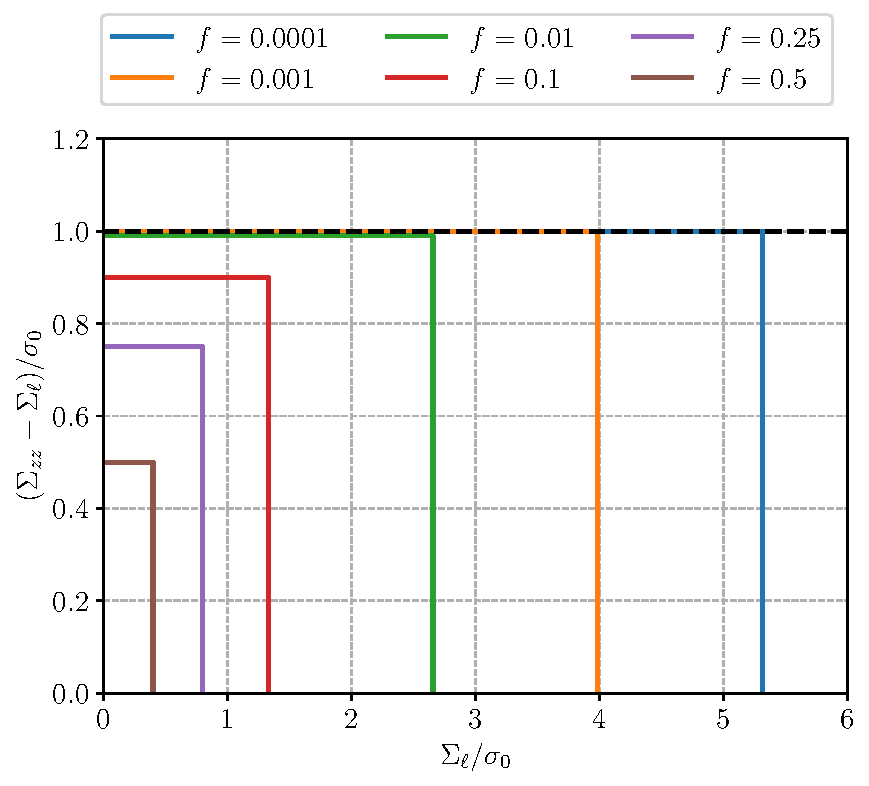
\includegraphics[width=0.6\textwidth]{Gurson_cylinder_approx}
\captionof{figure}{Estimation du critère macroscopique pour différentes valeurs de $f$. Le critère est exact est nécessairement situé à l'intérieur de cette estimation.}\label{fig:estimation}
\end{R_figure}
\end{solution}
\end{questions}

\section{Expression dans le cas général}
Par symétrie du critère, on se restreint ici à $A, B\geq 0$. Dans le cas général, il est possible de montrer que:
  \begin{align}
    \Pi(\td{D}) &= \sigma_0 A \left(\lambda M(\lambda)+N(\lambda)\right) \ \ \ \ \ \mathrm{avec} \ \ \ \ \ \lambda = \frac{2B}{\sqrt{3}Ab^2} \\
    M(\lambda) &=\mathrm{asinh}{\left( \frac{\lambda}{f} \right)} -\mathrm{asinh}{\left( \lambda \right)}\\
    N(\lambda) &= \sqrt{1 + \lambda^2} - \sqrt{f^2 + \lambda^2}
  \end{align}
On note en particulier $\lambda$ dépend de $\td{D}$ à travers $A$ et $B$ et que $\boxed{N'(\lambda)= -\lambda M'(\lambda)}$.

\begin{questions}
\question En explicitant l'Eq.~\eqref{eq:plastic-boundary}, montrer que les états de contrainte $\tSigma^*$ à la frontière du domaine sont donnés par:
  \begin{equation}
    \frac{\Sigma_{zz}^* - \Sigma_\ell^*}{\sigma_0} = N(\lambda)
\end{equation}  
    \begin{equation}
    \frac{\Sigma_\ell^*}{\sigma_0} = \frac{M(\lambda)}{\sqrt{3}}
\end{equation}  
\begin{solution}
$\td{D}$ est à présent paramétré par $A$ et $\lambda$. Ainsi, le travail des efforts extérieurs devient:
$$\tSigma \cdot \td{D} = \sqrt{3}A\lambda\Sigma_\ell + (\Sigma_{zz}-\Sigma_\ell)A.$$
Pour les états de contrainte situés à la frontière du domaine, on a $\tSigma^* \cdot \td{D} = \Pi(\td{D})$ ce qui donne:
$$  \sqrt{3}\lambda\Sigma_\ell^* + \Sigma_{zz}^*-\Sigma_\ell^* = \sigma_0 \left(\lambda M(\lambda)+N(\lambda)\right)$$
En dérivant par rapport à $\lambda$ à gauche et à droite, on obtient:
$$ \sqrt{3}\Sigma_\ell^* = \sigma_0 M(\lambda)+ \sigma_0(\lambda M'(\lambda)+N'(\lambda))$$
Comme le dernier terme s'annule par construction, on a bien:
$$\frac{\Sigma_\ell^*}{\sigma_0} = \frac{M(\lambda)}{\sqrt{3}}$$
D'où on déduit de l'expression précédente que:
$$\Sigma_{zz}^*-\Sigma_\ell^* = \sigma_0 N(\lambda)$$
\end{solution}
%donner les expressions de $\Sigma_{xx}$ et $\Sigma_{zz}$ en fonction de $D_{xx}$ et $D_{zz}$.\\
  
\question En combinant les expressions précédentes, montrer que:
  \begin{equation}
   \Phi\left( \tSigma     \right)  = \left(  \frac{\Sigma_{zz} - \Sigma_\ell}{\sigma_0} \right)^2 + 2f \cosh{\left(  \sqrt{3} \frac{\Sigma_\ell}{\sigma_0} \right)} - (1 + f^2) = 0
\label{eq4}
  \end{equation}  
  \textit{On rappelle que: 
  \begin{align*}
  \cosh(a-b)&=\cosh(a)\cosh(b)-\sinh(a)\sinh(b) \\
  \cosh(\mathrm{asinh}(x)) &= \sqrt{1+x^2}.
  \end{align*}}
\begin{solution}
On a:
\begin{align*}
\cosh{\left(  \sqrt{3} \frac{\Sigma_\ell}{\sigma_0} \right)} &= \cosh{\left[\mathrm{asinh}{\left( \frac{\lambda}{f} \right)}\right]}\cosh[\mathrm{asinh}{(\lambda)}] - \sinh{\left[\mathrm{asinh}{\left( \frac{\lambda}{f} \right)}\right]}\sinh[\mathrm{asinh}{(\lambda)}]\\
&= \sqrt{\left(\frac{\lambda}{f} \right)^2+1}\sqrt{\lambda^2+1} - \frac{\lambda^2}{f}
\end{align*}
En remarquant que:
$$\left(  \frac{\Sigma_{zz} - \Sigma_\ell}{\sigma_0} \right)^2 = N(\lambda)^2 = 1+\lambda^2+f^2+\lambda^2 -2\sqrt{1+\lambda^2}\sqrt{f^2+\lambda^2}$$
on vérifie bien l'expression demandée.\\

On constate que le critère obtenu est anisotrope, plus précisément, isotrope transverse. Cette anisotropie est induite par la géométrie du milieu poreux qui présente cette classe de symétrie matérielle. $\Sigma_{\ell}$ and $\Sigma_{zz}-\Sigma_{\ell}$ sont en réalité deux invariants pour l'isotropie transverse.
\end{solution}
\end{questions}

\section{Etude du critère}
L'Eq.~\eqref{eq4} correspond au critère de plasticité pour le matériau poreux recherché, dont il convient de vérifier la pertinence en étudiant les cas limites.\\

\begin{questions}
\question Que devient l'Eq.~\eqref{eq4} dans la limite $f \to 0$ ? Et dans la limite $f \to 1$ ?
\begin{solution}
Lorsque $f\to 0$, il n'y a plus de pore et on retombe sur le critère de von Mises de la matrice. \`A la limite $f\to 1$, compte-tenu du fait que $\cosh(x)\geq 1$, on constate qu'il n'est plus possible de vérifier le critère sauf si $\tSigma=0$.
Cela est cohérent avec les deux estimations précédentes qui dégénèrent lorsque $f\to 1$.
\end{solution}

La figure \ref{fig:Gurson_crit} trace le critère dans le plan $(\Sigma_\ell, \Sigma_{zz} - \Sigma_\ell)$ pour différentes valeurs de porosité.

\begin{figure}
\begin{center}
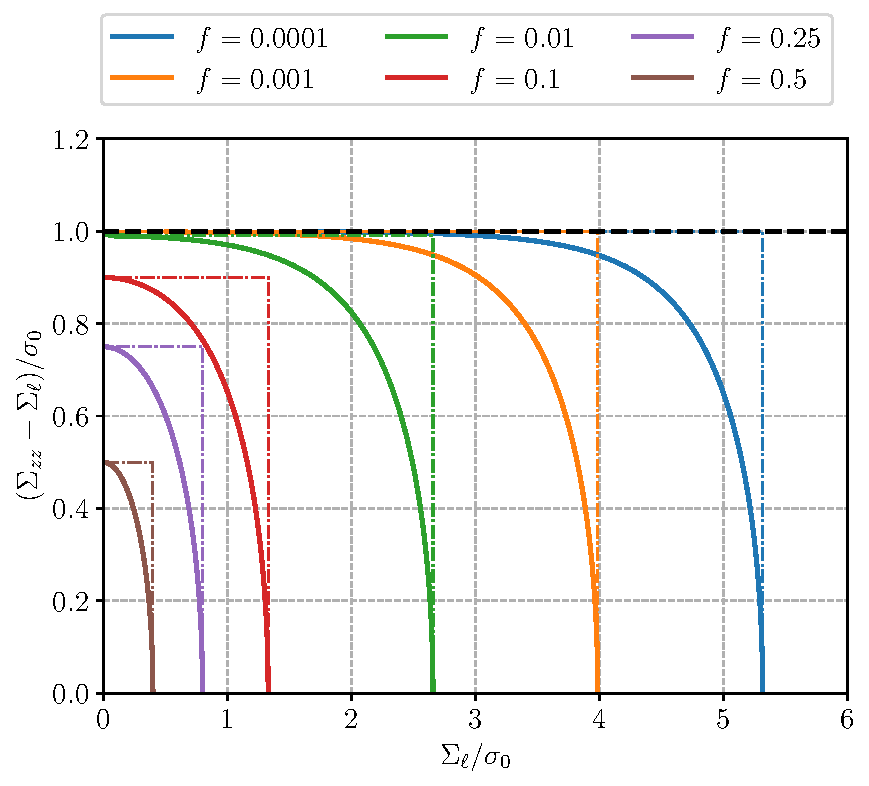
\includegraphics[width=0.5\textwidth]{Gurson_cylinder}
\end{center}
\caption{Critère de Gurson dans le plan $(\Sigma_\ell, \Sigma_{zz} - \Sigma_\ell)$ pour différentes valeurs de porosité. En noir pointillés: le critère de von Mises de la matrice. En couleurs pointillées: les estimations de la section 2.}
\label{fig:Gurson_crit}
\end{figure}

Le critère de plasticité obtenu doit être accompagné d'une loi d'écoulement, de la même manière que pour la plasticité de von Mises (Eq.~\ref{eq200}). Hill \cite{hill}, puis Rice \cite{rice} et enfin Gurson \cite{gurson} dans le cas des matériaux poreux , ont montré, grâce au principe de dissipation maximale, que la loi de normalité est conservée au niveau macroscopique lors du changement d'échelle. On a donc:

  \begin{equation}
     \td{D} = \dot{\Lambda} \frac{\partial \phi(\tSigma)}{\partial \tSigma},  \quad \dot{\Lambda}\geq 0
  \end{equation}
où $\dot{\Lambda}$ est le multiplicateur plastique de la loi de plasticité macroscopique.

\question Déterminer $D_{xx}$, $D_{zz}$ en fonction de $\Sigma_\ell$, $\Sigma_{zz}$.
 \begin{solution}
 On a:
\begin{align*}
\frac{\partial \phi(\tSigma)}{\partial \tSigma} &= \frac{\partial \phi(\tSigma)}{\partial \Sigma_\ell}\frac{\partial \Sigma_\ell}{\partial \tSigma} + \frac{\partial \phi(\tSigma)}{\partial \Sigma_{zz}}\frac{\partial \Sigma_{zz}}{\partial \tSigma}\\
 &= \frac{\partial \phi(\tSigma)}{\partial \Sigma_\ell}\dfrac{1}{2}\td{1}_p + \frac{\partial \phi(\tSigma)}{\partial \Sigma_{zz}}\td{e}_z\otimes\td{e}_z
\end{align*}
On a donc:
 $$D_{zz} = \dot{\Lambda}\dfrac{\partial \phi(\tSigma)}{\partial \Sigma_{zz}} = 2\dot{\Lambda}\dfrac{\Sigma_{zz}-\Sigma_\ell}{\sigma_0^2} \quad (=0\text{ si } \Sigma_{zz}=\Sigma_\ell)$$
et
$$D_{xx} = \dfrac{\dot{\Lambda}}{2}\dfrac{\partial \phi(\tSigma)}{\partial \Sigma_\ell} = -\dot{\Lambda}\dfrac{\Sigma_{zz}-\Sigma_\ell}{\sigma_0^2} +  \dot{\Lambda}\dfrac{\sqrt{3}f}{\sigma_0} \sinh{\left(  \sqrt{3} \frac{\Sigma_\ell}{\sigma_0} \right)} $$
 \end{solution} 


 \question Dans le cadre de la modélisation de la rupture ductile, l'évolution de la porosité $f$ est particulièrement d'intérêt. Montrer que $\dot{f} = (1 - f) \mathrm{tr} (\td{D})$. Donner son expression en fonction de $\Sigma_\ell,\Sigma_{zz}$ et $D_{zz}$.
\begin{solution}
La porosité est donnée par $f=V_f/V$ où $V_f$ est le volume des pores et $V=V_f+V_m$ le volume total. La matrice étant incompressible et en l'absence de nucléation, on a $\dot{V}_m=0$ et donc $\dot{V}=\dot{V}_f$. Ainsi:
$$\dot{f} = \dfrac{\dot{V}_f}{V}-\dfrac{V_f\dot{V}}{V^2} = \dfrac{\dot{V}}{V}\left(1-\dfrac{V_f}{V}\right)$$
Enfin, par définition du taux de déformation, $\mathrm{tr}( \td{D}) =  \dfrac{\dot{V}}{V}$ de sorte que:
$$\dot{f}=(1-f)\mathrm{tr}(\td{D}) = (1-f)(2D_{xx}+D_{zz})$$

Grâce aux relations précédentes, on a:
$$\dot{f} = (1-f)\dot{\Lambda}\dfrac{2\sqrt{3}f}{\sigma_0} \sinh{\left(  \sqrt{3} \frac{\Sigma_\ell}{\sigma_0} \right)} $$
De plus:
$$\dot{\Lambda}= \dfrac{D_{zz}\sigma_0^2}{2(\Sigma_{zz}-\Sigma_\ell)}$$
soit:
$$\dot{f} = (1-f)f\dfrac{\sqrt{3}\sigma_0}{\Sigma_{zz}-\Sigma_\ell}D_{zz}$$
\end{solution}
\end{questions}

\section{Extension aux matériaux anisotropes}
Le critère de plasticité pour matériaux poreux obtenu est pertinent dans le cas des matériaux isotropes. Le matériau caractérisé dans les travaux pratiques (alliage X100) est orthotrope et peut être modélisé, en l'absence de porosité, par la plasticité de Hill:
\begin{equation}
  \phi\left( \sigma   \right) =  \sigma_{eq}^H - \sigma_0 \leq 0 \quad \text{avec } \sigma_{eq}^H = \sqrt{ \td{\sigma} \cdot \tq{A} \cdot \td{\sigma}}
  \label{eq100}
\end{equation}
Le tenseur $\tq{A}$ contient les informations concernant l'anisotropie du matériau. En notation de Mandel, ces tenseurs sont représentés par les matrices suivantes dans les axes d'orthotropies:
\begin{equation}
  \tsigma = \begin{pmatrix}
    \sigma_{11} \\
    \sigma_{22} \\
    \sigma_{33} \\
    \sqrt{2}\sigma_{12} \\
    \sqrt{2}\sigma_{13} \\
    \sqrt{2}\sigma_{23} \\
  \end{pmatrix} \hspace{2cm}
  \tq{A} = \begin{pmatrix}
    F + H & -F & -H & 0 & 0 & 0 \\
    -F & G+ F & -G & 0 & 0 & 0 \\
    -H & -G & G+H & 0 & 0 & 0 \\
    0 & 0 & 0 & L & 0 & 0 \\
    0 & 0 & 0 & 0 & M & 0 \\
    0 & 0 & 0 & 0 & 0 & N \\
    \end{pmatrix}
\end{equation}
Pour $F = G = H = 1/2$ et $L = M = N = 3/2$, le critère de Hill correspond au critère de von Mises.
% On considère ici le cas isotrope transverse d'axe $\td{e}_z$. Dans ce cas, $G=H$ et $L=G+2F$.\\
%La loi d'écoulement plastique associée permet d'obtenir le taux de déformation plastique:
%\begin{equation}
%  \td{d} = d_{eq} \frac{\tq{A}}{\sigma_0}  \hspace{2cm} d_{eq} = \sqrt{\td{d} \cdot \tq{B} \cdot \td{d} }
%  \label{eq10}
%\end{equation}
%où les paramètres du tenseur $\tq{B}$ sont reliés à ceux de $\tq{A}$ par les relations donnés en Annexe.\\
%\begin{itemize}
%  \question Quels paramètres est-il possible d'obtenir à partir des résultats expérimentaux ?\\
%\end{itemize}

Il est possible de conduire la même démarche d'analyse limite que dans le cas isotrope pour prendre en compte l'effet de la porosité, ce qui conduit au critère de plasticité suivant \cite{benzerga}:
  \begin{equation}
   \Phi\left( \Sigma     \right)  = \left(  \frac{\Sigma_{eq}^H}{\sigma_0^2} \right)^2 + 2f \cosh{\left(  \frac{\sqrt{3}}{h_m} \frac{\Sigma_\ell}{\sigma_0} \right)} - (1 + f^2) = 0
\label{eq5}
  \end{equation} 

avec $h_m = \sqrt{\dfrac{3}{2}}\sqrt{\dfrac{H+G}{4(FG+FH+GH)} + \dfrac{1}{2L}}$.
\begin{questions}
\question Dans quelle situation particulière de symétries matérielles est-il raisonnable de considérer le même champ de vitesse qu'en \eqref{eq:champ-vitesse} ?
\begin{solution}
Le champ précédent suppose une invariance par rotation autour de l'axe $z$. Ce champ peut donc être utilisé dans le cas particulier de l'isotropie transverse d'axe $z$. Dans ce cas, on doit avoir $G=H$ et $L=G+2F$. On a alors:
$$h_m = \sqrt{\dfrac{3/2}{G+2F}}.$$

On remarquera que même si le matériau n'est pas isotrope transverse, il est toujours possible d'utiliser ce champ de vitesse qui reste admissible. On obtiendra alors une borne extérieure du critère dont il conviendra de vérifier si elle est de bonne qualité ou non, soit en considérant un champ de vitesse plus compliqué, soit par comparaison à des simulations numériques.
\end{solution}
    \question \`A partir de l'expression précédente, commenter l'effet de l'anisotropie sur la plasticité des matériaux poreux.
\begin{solution}
On constate que l'anisotropie impacte plusieurs aspects du critère. Premièrement, l'anisotropie impacte la définition de la norme équivalente $\Sigma_{eq}^H$. De plus, si l'on trace le critère dans le plan $(\Sigma_\ell,\Sigma_{eq}^H)$, l'anisotropie impacte, via le facteur $h_m$ la limite suivant l'axe $\Sigma_\ell$. Par conséquent, ce même facteur aura également un effet sur l'évolution de la porosité puisque, si l'on reprend les mêmes calculs que précédemment pour la règle de normalité, on aura notamment:
$$\mathrm{tr}(\td{D}) = \dot{\Lambda}\dfrac{2\sqrt{3}f}{h_m\sigma_0} \sinh{\left(  \sqrt{3} \frac{\Sigma_\ell}{h_m\sigma_0} \right)} = \dfrac{\dot{f}}{1-f}$$
On voit donc que l'effet de l'anisotropie impacte également la loi d'évolution de la porosité.
\end{solution}
\end{questions}

\section*{Calcul différentiel en coordonnées cylindriques}
\textbf{Gradient d'un champ vectoriel} $\td{v}(r,\theta,z)=v_r(r,\theta,z)\td{e}_r+v_\theta(r,\theta,z)\td{e}_\theta+v_z(r,\theta,z)\td{e}_z$
$$ \gradient{v} = \begin{bmatrix}
\dfrac{\partial v_r}{\partial r} & \dfrac{1}{r}\left(\dfrac{\partial v_r}{\partial \theta} - v_\theta\right) & \dfrac{\partial v_r}{\partial z} \\
\dfrac{\partial v_\theta}{\partial r} & \dfrac{1}{r}\left(\dfrac{\partial v_\theta}{\partial \theta} + v_r\right) & \dfrac{\partial v_\theta}{\partial z} \\
\dfrac{\partial v_z}{\partial r} & \dfrac{1}{r}\dfrac{\partial v_z}{\partial \theta} & \dfrac{\partial v_z}{\partial z} \\
\end{bmatrix}_{(\td{e}_r,\td{e}_\theta,\td{e}_z)}$$

\begin{thebibliography}{9}
\bibitem{hill}
Hill, R. (1967). The essential structure of constitutive laws for metal composites and polycrystals. Journal of the Mechanics and Physics of Solids, 15(2), 79-95.
\bibitem{rice} 
Rice, J. R. (1971). Inelastic constitutive relations for solids: an internal-variable theory and its application to metal plasticity. Journal of the Mechanics and Physics of Solids, 19(6), 433-455.
\bibitem{gurson}
Gurson, A.L. (1975). Plastic flow and fracture behaviour of ductile materials incorporating void nucleation, growth and interaction. PhD thesis. Brown University, Providence, USA.
\bibitem{benzerga}
Benzerga, A. A.,   \& Besson, J. (2001). Plastic potentials for anisotropic porous solids. European Journal of Mechanics-A/Solids, 20(3), 397-434.


\end{thebibliography}

\end{document}
